\documentclass[12pt,a4paper]{scrreprt}

\usepackage{fontspec}
\usepackage{geometry}
\usepackage{mathtools}
\usepackage[english]{babel}
\usepackage{longtable,booktabs}
\usepackage{grffile}
\usepackage{graphicx}
\usepackage{titlesec}
\usepackage{capt-of}
\usepackage{newtxtext,newtxmath}

%\setlength{\leftskip}{25pt}
\makeatother
% Make links footnotes instead of hotlinks
%\renewcommand{\href}[2]{#2\footnote{\url{#1}}}

% No paragraph indentation
% and set space between paragraphs
\setlength{\parindent}{0pt}
\setlength{\parskip}{0.5em plus 1pt minus 1pt}
\setlength{\emergencystretch}{3em} % Prevent overfull lines
% Chapter: 0, section: 1, subsection: 2 etc
\setcounter{secnumdepth}{2}
\setcounter{tocdepth}{2}

\begin{document}
\pagenumbering{roman}
\begin{titlepage}
  \begin{center}

    
\includegraphics[width=40mm]{tu}\par\vspace{0.8cm}
    \textsc{\LARGE Tribhuwan University}\\[1cm]
    \textsc{\bfseries INSTITUTE OF ENGINEERING}\\
    \textsc{\bfseries PULCHOWK CAMPUS}\\
    \textsc{Pulchowk, Lalitpur}\\
    \vspace{0.8cm}

    \textsc{\Large A Case Study}\\[0.5cm]
    \textsc{On}\\
    {\huge \bfseries Paila Technology\\[0.4cm]}

    \vfill
    {\Large \bfseries Submitted By:\\}
    \noindent\makebox[\textwidth]{%
      \begin{tabular}{lr}%
        Aashutosh Poudel & \texttt{072BCT502}\\
        Dinesh Bhattarai & \texttt{072BCT512}\\
        Krishna Upadhyay & \texttt{072BCT517}\\
        Rupesh Shrestha  & \texttt{072BCT530}\\
        Simon Dahal  & \texttt{072BCT538}\\
        Yogesh Rai  & \texttt{072BCT548}\\
    \end{tabular}}\\[1cm]

    {\Large \bfseries Submitted To:\\}
    \textsc{Department of Mechanical Engineering} \\
    \textsc{Lalitpur, Nepal}
    \\[1cm]

    \vfill

    {\large \today}

  \end{center}
\end{titlepage}

\chapter*{Acknowledgements}
\thispagestyle{empty}
We would like to express our deepest gratitude to Prof. Shyam Krishna Joshi, honorable Professor for Organization and Management course, for his invaluable assistance, proper guidance and immense support to make us understand the core concept of Organization and Management and also encouraging us to do this case study on field.

Furthermore, we would also like to express our gratitude to Paaila Technology for not only allowing us to perform the study but also for helping us in all manners possible. Specifically, we would like to thank Mr. Wasim Akram Khan, Co-founder and Software Engineer and Mr. Dip Kamal Bhusal, CCO and Co-founder at Paaila Technology for dedicating their invaluable time and efforts towards this study and assisting us in the endeavor. Lastly, we would like to thank all our seniors, friends and family members for their support and suggestions.

- Team Members

\clearpage
\tableofcontents
\listoffigures
\listoftables
\clearpage
\pagenumbering{arabic}

\chapter{Introduction}
"Paila Technology", first of its kind in Nepali market, is a robotics and AI startup established on December 12, 2016 by Bijay Raut along with five other engineering graduates from IOE, Pulchowk Campus. The company started with a core team of seven members and the team has grown ever since. The company aims to produce world class robotics and industrial automation products that are suitable for businesses.
The company started with Automatic Dhara, automation for homes and have now transitioned into robotics by presenting their flagship project Pari, a robot for Nepal SBI Digital InTouch branch at Durbar Marg. Pari is a product that created a new market segment of robotics in Nepali market.

Paila is an entrepreneurial venture started with the prime motive to meet the demands of the market by developing a viable business model around some innovative products, services processes and platforms integrated with Artificial Intelligence and Robotics. The business model was a huge success in context of Nepal and the customerbase of the company is on rise. In a short span of time, the company has delivered products and services to some of the biggest names in the country including SBI Nepal Limited, nLocate, Gyani Traders and more to count.

\section{Vision}
The primary vision of "Paaila" can be considered as production of human friendly robots and to aid in the technological development of the country by embracing AI in different fields. It wants to aid other companies in integrating AI in their products as well to make AI and robotics available to everyone.

\section{Objectives}
The major objectives set by the company are:
\begin{enumerate}
  \item Be the best workplace for robotics and AI
  \item Be the best option for businesses seeking robotics Services
  \item Help Nepali companies integrate AI into their products and services.
\end{enumerate}

\chapter{Products and Services}
\section{Variable Frequency Drive}
\begin{enumerate}
  \item Introduction \\
    A Variable Frequency Drive (VFD) is a type of motor controller that drives an electric motor by varying the frequency and voltage supplied to the electric motor. Other names for a VFD are variable speed drive, adjustable speed drive, adjustable frequency drive, AC drive, and inverter. As the application's motor speed requirement change, the VFD can simply turn up or down the motor speed to meet the speed requirement.

  \item Working\\
    The first stage of a Variable Frequency AC Drive, or VFD, is the Converter. The converter is a comprised of six diodes, which are similar to check values used in plumbing systems. They allow current to flow in only one direction; the direction shown by the arrow in the diode symbol. For example, whenever A-phase voltage (voltage is similar to pressure in plumbing systems) is more positive than B or C phase voltages, then that diode will open and allow current to flow. When B-phase becomes more positive than A-phase, then the B-phase diode will open and the A-phase diode will close. The same is true for the 3 diodes on the negative side of the bus. Thus, we get six current "pulses" as each diode opens and closes. This is called a "six-pulse VFD", which is the standard configuration for current Variable Frequency Drives.

    \begin{center}
        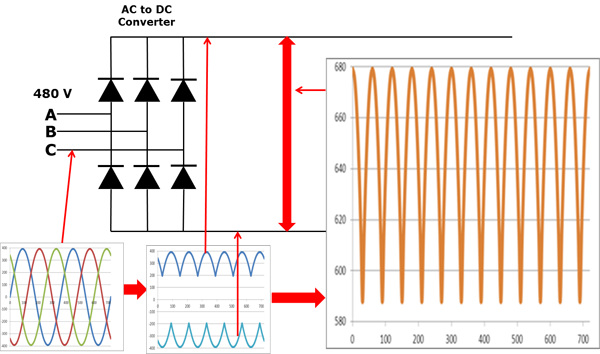
\includegraphics{vfd1}
        \captionof{figure}{Converter in a VFD}
    \end{center}

    If the drive is operating on a 480V power system, then the 480V rating is "rms" or root-mean-squared. The peaks on a 480V system are 679V. The VFD dc bus has a dc voltage along with an AC ripple. The voltage runs between approximately 580V and 680V.

    \begin{center}
        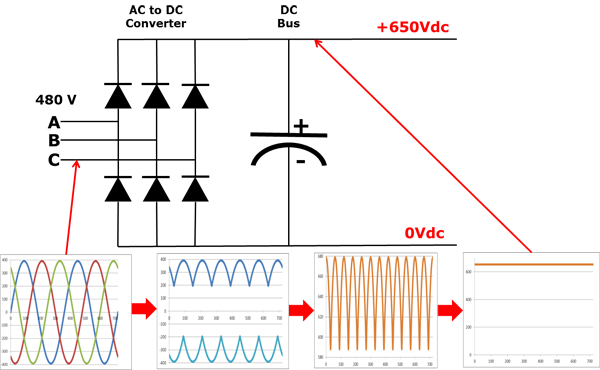
\includegraphics{vfd2}
        \captionof{figure}{Converter with DC Bus in a VFD}
    \end{center}

    A capcitor is added to get rid of the AC ripple on the DC bus. A  capacitor operates in a similar fashion to a reservoir or accumulator in a plumbing system. This capacitor absorbs the ac ripple and delivers a smooth dc voltage. The AC ripple on the DC bus is typically less than 3 Volts. Thus, the voltage on the DC bus becomes "approximately" 650VDC. The actual voltage will depend on the voltage level of the AC line feeding the drive, the level of voltage unbalance on the power system, the motor load, the impedance of the power system, and any reactors or harmonic filters on the drive. \\

    The diode bridge converter that converts AC-to-DC, is sometimes just referred to as a converter. The converter that converts the dc back to ac is also a converter, but to distinguish it from the diode converter, it is usually referred to as an "inverter". It is common in the industry to refer to any DC-to-AC converter as an inverter.

    \begin{center}
        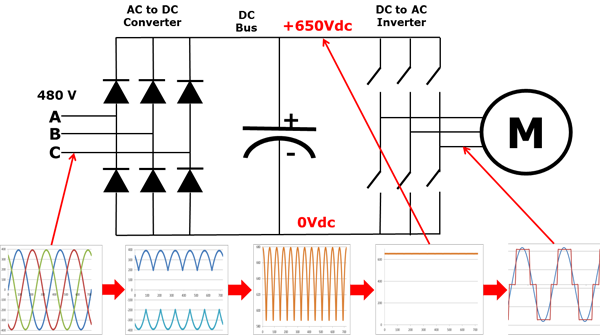
\includegraphics{vfd3}
        \captionof{figure}{Converter, DC Bus, and inverter in a VFD}
    \end{center}

    When one of the top switches in the inverter is closed, that phase of the motor is connected to the positive dc bus and the voltage on that phase becomes positive. When one of the bottom switches in the converter is closed, that phase is connected to the negative dc bus and becomes negative. Thus, any phase on the motor can be made positive or negative at will and can thus generate any frequency. Also, any phase can be made positive, negative, or zero.

    \begin{center}
      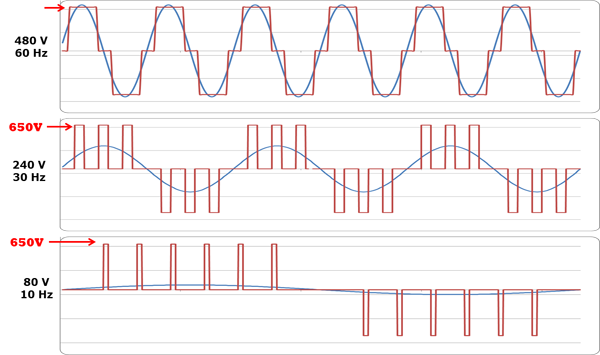
\includegraphics{vfd4}
      \captionof{figure}{Output response of a VFD}
    \end{center}

    The output from the VFD is of "rectangular" wave form. VFD's do not produce a sinusoidal output. This rectangular waveform would not be a good choice for a general purpose distribution system, but is perfectly adequate for a motor.

  \item Benefits
    \begin{itemize}
      \item Electric motor systems are responsible for more than 65\% of the power consumption in industry. Optimizing motor control systems using VFDs can reduce energy consumption and energy costs.
      \item Using VFDs, equipments can be operated at optimimum and efficient speeds, thereby extending the equipment life and reducing maintenance costs.
    \end{itemize}

  \item VFDs by Paila Technology
    \begin{itemize}
      \item Current Market in Nepal
        \begin{itemize}
          \item VFDs for \textit{Allo} thread producing machine
          \item VFDs for changing speed of DC motors in tempos
          \item VFDs for automatic brick producing machines
        \end{itemize}

      \item Features
        \begin{itemize}
          \item Customizable for different applications
          \item Production against possible drive failures
          \item Quality support and maintenance
          \item Compatible with single phase supply
          \item Made for Nepali Industries
        \end{itemize}

      \item Technical Specification
        \begin{center}
          \begin{tabular}{|l|l|}
            \hline
            Parameters & Values \\
            \hline
            Input Voltage & 380 to 480V 3ph or 230V single phase \\
            Input Frequency & 50Hz or 60Hz \\
            Output Voltage & 0 to rated line voltage \\
            Output Frequency & 0.5Hz to 200Hz \\
            Switching Frequency & 3kHz to 12kHz \\
            Rated Power & 0.5HP to 15 HP \\
            Control Method & Linear V/f \\
            Display & 7-segment or Alphanumeric LCD \\
            Digital Inputs & 5V DC optically isolated \\
            Analog Inputs & 0 to 5V \\
            \hline
          \end{tabular}
        \end{center}
    \end{itemize}
    Resources: https://www.vfds.com/blog/what-is-a-vfd
\end{enumerate}
\chapter{Organization Structure}
\chapter{Personnel Management}
\section{Recruitment, Selection and Training}
\section{HR Divisions}
\subsection{Mechanical Division}
\subsection{Embedded Division}
\subsection{Language Processing}
\subsection{Operation Management}

\section{Motivation}

\chapter{Finance Management}
\chapter{Software Engineering Methodology}

\chapter{Organizational Challenges}
\section{Lack of expertise and difficulty to retain them}
\section{Lack of raw materials}
\section{Insufficient training data-sets}

\chapter{Recommendation}
\section{Outsourcing}
\section{Extending HR base for better responsibility division}

\chapter{Conclusion}
\chapter*{References}
\bibliography{bibliography}
\end{document}
